\section{监测设计}
\label{sec:design}

方差结构可以回答两个设计问题，即总预算固定时期数与单期规模如何取舍，以及规模较小时如何可靠地判断疫情是否在增长。

\subsection{多期预算分配}
\label{sec:design-budget}

设共观测 $T$ 期，每期预计报告 $m$ 例，总量 $B=Tm$ 固定。用各期估计的平均值 $T^{-1}\sum_t\widehat R_t$ 估计 $\Rbar$。

\begin{proposition}[多期分配]
\label{prop:allocation}
在 H1--H4 下，若各期 $R_t$ 相互独立，则
\begin{equation}
  \frac{1}{T^2}\Var({\textstyle\sum_{t=1}^{T}}\widehat R_t)=\frac{v_R}{T}+\frac{A}{B}.
  \label{eq:alloc-indep}
\end{equation}
若 $R_t$ 服从系数为 $r\in(0,1)$ 的平稳一阶自回归过程，规模项仍为 $A/B$，环境项变为
\begin{equation}
  \frac{v_R}{T}\cdot\frac{1+r}{1-r}-\frac{2r(1-r^T)\,v_R}{T^2(1-r)^2}.
  \label{eq:alloc-ar}
\end{equation}
两种情形下，方差都随 $T$ 严格递减。
\end{proposition}

总量固定时，规模项 $A/B$ 与如何切分无关，环境项则随期数增多而下降。所以只看方差，期数越多越好。式~\eqref{eq:alloc-ar} 是一阶自回归过程部分和方差的精确表达式\citep{hamilton1994time}。常用的有效期数近似 $T_{\mathrm{eff}}=T(1-r)/(1+r)$ 只保留了方括号内第一项，总会高估环境项。$r=0.8$ 时，$T=26$ 高估 20.5\%，$T=10$ 高估 65.8\%。近似只在 $T\gg 2r/(1-r^2)$ 时可用。

实际切分还受整数约束。每期需要 $n=B/(\rho T)$ 名感染者，因此 $T$ 必须整除 $B/\rho$。例如 $B=30$、$\rho=0.25$ 时，$B/\rho=120$，可行的 $T$ 为 120 的 16 个因数；$\rho=0.7$ 时 $B/\rho$ 非整数，可行集为空，只能放宽总量。

期数不能无限增加，因为每多观测一期都有固定成本，例如启动一轮调查或维持一个报告周期。设每期固定成本为 $c_0$，每例预计报告病例的边际成本为 $c_1$，总经费为 $\mathcal B$，于是 $T=\mathcal B/(c_0+c_1m)$。

\begin{corollary}[最优单期规模]
\label{cor:optimal}
在命题~\ref{prop:allocation} 的独立情形下，估计方差为 $f(m)=(c_0+c_1m)(v_R+A/m)/\mathcal B$。当 $c_0>0$ 时，它在下式处取最小值
\begin{equation}
  m^*=\sqrt{\frac{c_0}{c_1}\,\mx},\qquad
  f(m^*)=\frac{(\sqrt{c_0v_R}+\sqrt{c_1A})^2}{\mathcal B}.
  \label{eq:optimal-m}
\end{equation}
若 $\mathcal B<c_0+c_1m^*$，约束 $T\geq1$ 起作用，最优解取 $T=1$；若 $c_0=0$，最优解为 $m\to0$。
\end{corollary}

最优单期规模是成本比 $c_0/c_1$ 与交叉点 $\mx$ 的几何平均。这与两阶段抽样的费用分配是同一个问题\citep{cochran1977sampling}。期数 $T$ 对应初级单元数，$v_R$ 对应初级单元间方差，$A$ 对应单元内方差，$c_0$ 与 $c_1$ 分别对应初级单元和次级单元的单位成本。

按第~\ref{sec:empirical-early}~节的情景参数，$\mx$ 在 21.3--49.2。$c_0/c_1=10$ 时 $m^*$ 为 14.6--22.2，$c_0/c_1=100$ 时为 46.1--70.1。在图~\ref{fig:variance} 的参数下（$\mx=53.1$），两种成本比对应的 $m^*$ 为 23.0 和 72.9。

连续解需要取整后才能执行。取图示参数，$c_0=100$，$c_1=1$，$\mathcal B=600$，连续解为 $m^*=72.86$，对应的 $T$ 不是整数。逐个比较整数 $T$ 后，最优方案是 $T=3$、$m=100$，方差为 0.02041。若环境服从一阶自回归，$m^*$ 应乘以约 $\sqrt{(1-r)/(1+r)}$，即正相关使最优方案偏向更多、更小的期。仍取图示参数与 $c_0/c_1=100$，$r=0.5$ 时精确最优与近似值分别为 42.9 和 42.1，$r=0.8$ 时为 25.0 和 24.3。

\subsection{增长检验}
\label{sec:design-test}

监测中最常见的判断是疫情是否在增长，即检验 $H_0\colon R_t\leq1$ 对 $H_1\colon R_t>1$。这是目标Ⅰ层面的问题。

\begin{proposition}[精确增长检验]
\label{prop:test}
在 H1--H3 下，$C_t$ 的分布族关于 $R_t$ 具有单调似然比。令 $c_\alpha$ 为满足 $P_{R_t=1}(C_t\geq c)\leq\alpha$ 的最小整数，检验在 $C_t\geq c_\alpha$ 时拒绝 $H_0$。该检验有以下三条性质。
\begin{enumerate}[label=(\roman*)]
  \item 第一类错误概率在 $R_t\leq1$ 上的上确界在 $R_t=1$ 处取得，实际水平 $\alpha^*\leq\alpha$。
  \item 该检验在水平 $\alpha^*$ 下一致最优；加入随机化的 Karlin--Rubin 检验恰好达到水平 $\alpha$，并在该水平下一致最优。
  \item 在 $R_t=1+\delta$ 处的功效为：
  \begin{equation}
    \pi(n,\delta)=1-F_{\NB}(c_\alpha-1;\ nk,\ k/[k+\rho(1+\delta)]).
    \label{eq:power}
  \end{equation}
\end{enumerate}
\end{proposition}

命题~\ref{prop:test} 是单调似然比族上的标准结论\citep{karlin1956theory, lehmann2005testing}。它依赖 $k$ 已知；若 $k$ 用数据估计，水平不再有精确保证。

实际工作中常用正态近似的 Wald 检验，即把 $(\widehat R_t-1)/\sqrt{V_0}$ 与正态分位数比较，其中 $V_0=1/(\rho n)+1/(kn)$ 是 $R_t=1$ 时的方差。该检验的实际水平同样可以用负二项分布函数精确算出。图~\ref{fig:test}a 显示，小规模时 Wald 检验系统性地超过名义水平。$k=0.1$、$m=5$ 时实际水平为 7.81\%；在 $m<40$ 的范围内，$k=0.1$、$0.35$ 和 $1$ 的最大实际水平分别为 8.03\%、8.75\% 和 10.40\%。精确检验在整个网格上的最大水平为 0.05000，没有超出名义水平。

功效随 $n$ 的变化呈锯齿状。$c_\alpha$ 只能取整数，每当它跳升一格，功效会短暂下降。以 $k=0.35$、$\delta=0.3$ 为例，$n$ 从 400 增加到 699 的过程中，功效下降了 82 次。因此只报告“首次达到 80\% 功效的规模”并不够，还要给出“此后始终保持 80\% 以上的规模”。在 $\rho=0.25$ 下，$k=0.35$ 时$\delta=0.15$、$0.3$、$0.5$ 依次为 2071/2107、568/581、229/235；$\delta=0.25$ 时，$k=1$ 为 568/585，$k=0.1$ 为 1660/1684。

这些数字与第~\ref{sec:variance-crossover}~节的结论形成对照。$k=0.35$ 时，要稳定检出 15\% 的增长，每期需要约 2107 名感染者，即 $m\approx527$ 例预计报告，是图示交叉点的十倍左右。对目标Ⅱ而言，规模过了 $\mx$ 收益就明显变小；对判断当期增长这类目标Ⅰ问题，规模的价值要大得多。

\begin{figure}[!tbp]
  \centering
  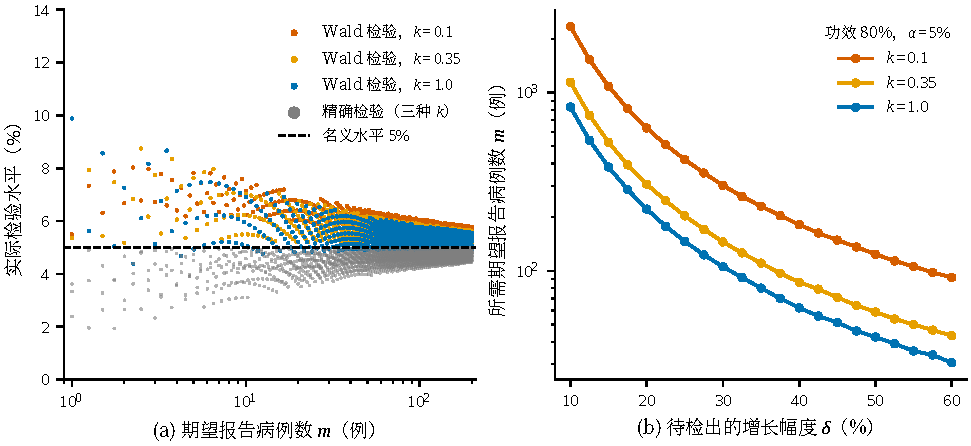
\includegraphics[width=\textwidth]{figures/fig_03_fig03_growth_test.pdf}
  \caption{增长检验的实际水平与所需规模，$\rho=0.25$，名义水平 5\%，全部由负二项分布函数精确计算。(a) Wald 检验（按 $k$ 着色）与精确检验（灰色）的实际水平随期望报告规模的变化。(b) 达到并保持 80\% 功效所需的期望报告规模与待检出增长幅度 $\delta$ 的关系。}
  \label{fig:test}
\end{figure}
